\chapter{Relativistic continuum mechanics}




\section{Lagrangian description of a field}
\index{Lagrangian description of a field}
\index{continuous mechanical system}
\index{field amplitudes}
A \textsl{continuous mechanical system}, also called a 
\textsl{field}, is a mechanical system which carries energy 
and has a  continuous-infinity of degrees of freedom.

In what follows, we consider a general 
\textsl{$n$-component field} which has  $n$ \textsl{field 
amplitudes} $\qam (x^\gka) $ ($\gkq = 1,2,3.\dots,n $) each 
of which is a differentiable function of the spacetime 
coordinates $x^\gka$ ($\gka=0,1,2,3 $). We may recall that 
we use the Greek  indices $\gka,\gkb,\gkg,\gkd,\dots$ for 
the spacetime range $0,1,2,3$  throughout this book. The 
only exception to this  convention is the Greek suffix 
$\gkq$ on the field amplitudes $\qam (x^\gka) $ and we use 
$\gkq$ exclusively for the special range  $\gkq = 
1,2,3,\dots,n $, that too in this chapter only.

\index{Lagrangian density}
The $n$-component field is characterised by its   
\textsl{Lagrangian density} $\EuScript{L} = \EuScript{L} 
(\qam , \qgr{\gka}, x^\gka)$ which is also simply called the 
field Lagrangian. It is a function of the  \textsl{the 
Lagrangian variables of the field}\index{Lagrangian 
variables},  namely, the field amplitudes $\qam$, their 
4-gradients   $\qgr{\gka}\equiv 
\dow_\gka\qam \equiv (\dow/\dow x^\gka) \qam $ and the  
spacetime coordinates $x^\gka$. A field is said to be a 
\textsl{closed system} \index{closed system} if its 
Lagrangian is not an explicit function of the 
spacetime coordinates $x^\gka$\footnote{Otherwise, \ie, if 
the spacetime coordinates 
$x^\gka$ do appear directly in $\EuScript{L}$, one calls the 
system an open-system.}\index{open system} in which case we 
may denote the Lagrangian as  
$\EuScript{L}=\EuScript{L}(\qam, \qgr{\gka})$. Our   
discussion is limited to such closed 
systems only. Also, we must note that the closed-system 
Lagrangian  $\EuScript{L} = \EuScript{L} (\qam , 
\qgr{\gka})$ that we consider, is ultimately a function of 
the spacetime coordinates $x^\gka$ through the field  
amplitudes and their gradients, as 'a function of  
functions'.  It may be useful to note that, the space  
coordinates $x^1,x^2$, and $x^3$, which are part of the 
$x^\gka$ on which the field amplitudes $\qam$ depend (in 
general), are the continuous analogues of the discrete 
indices $k$ labelling the  generalized coordinates 
$q_{_k}$ of a discrete mechanical  system with a finite 
number of degrees of freedom.

\section{Equations of motion}\index{Equations of motion}
The \textsl{equations of motion} of a closed, 
continuous,  mechanical system, also called its 
\textsl{field equations},\index{field equations} are the 
\textsl{Euler-Lagrange equations}\index{Euler-Lagrange 
equations} of the \textsl{fixed-boundary  variational 
problem}

\begin{figure}[H]
\begin{center}
\begin{tikzpicture}
%   \draw[help lines,step=.25,red] (-4,-4) grid (5,5) ;
%   \foreach \y in {-4,-3.5,...,5}
%     \draw (-4.2,\y) node[left]{\tiny\y} ;
%   \foreach \x in {-4,-3.5,...,5}
%     \draw (\x,-4.2) node[below]{\tiny\x} ;
\node at (0,0)
{\includegraphics[scale=.8]%
{src/images/lbk-graphics/region-omega-bw}};
\node at (-.5,-.25){$\Omega$};
\node at (1,-1.5) {$\Sigma$};
\end{tikzpicture}
\end{center}
\caption{}
\end{figure}
\begin{align} \label{rcm.1}
\delta\int_{\Omega}\EuScript{L}(\qam ,
\qgr{\gka})\,\dd^4 x =0,
\end{align}
where the independent variations $\delta q_{_\gkq}$ are 
\textsl{arbitrary} at  every event in $\Omega$ except on 
its 3-boundary $\Sigma$ where they  \textsl{vanish}.

As done elsewhere in this book, we  follow  the  summation 
convention here too. In particular,  summation from $1$ to 
$n$ over the repeated suffix $\gkq$, as well as summations 
over the range $0$ to $3$ over all repeated Greek indices, 
are implied. To obtain the Euler-Lagrange equations, 
\textsl{we vary $\qam$ and $\qgr{\gka}$ keeping the 
coordinates $x^\gka$, the domain $\Omega$ and  its boundary 
$\Sigma$ fixed}. Then, Eqn.\eqref{rcm.1} leads to
\begin{align}\label{rcm.2}
&0=\delta\int_{\Omega}\EuScript{L}\,\dd^4 x
=\int_{\Omega}\delta\EuScript{L}\,\dd^4x \notag\\&
=\int_{\Omega}\left(\frac{\dow \EuScript{L}}{\dow
\qam }\delta\qam  +\frac{\dow
\EuScript{L}}{\dow \qgr{\gka}}\delta\qgr
{\gka} \right)\,\dd^4 x
\notag\\& = \int_{\Omega}
\left(\frac{\dow \EuScript{L}}{\dow \qam} \delta\qam  
+\frac{\dow \EuScript{L}}{\dow
\qgr{\gka}}\dow_\gka (\delta q_{\gkq}) \right)\,\dd^4 x
 \notag\\ & =\int_{\Omega}\left(\frac{\dow 
\EuScript{L}}{\dow \qam }
 -\dow_\gka\left\{\frac{\dow \EuScript{L}}{\dow
\qgr{\gka}}\right\}\right)\delta\qam \dd^4
x \notag\\&\qquad\qquad+\int_{\Omega}\dow_\gka 
\left\{\frac{\dow 
\EuScript{L}} {\dow \qgr{\gka}}\delta\qam \right\}
\dd^4 x.
\end{align}

Using Gauss' theorem, the second integral on the last line
of Eqn.\eqref{rcm.2}  may be converted into the surface 
integral
\begin{align*}
\oint_\Sigma \left\{\frac{\dow \EuScript{L}}{\dow
\qgr{\gka}}\delta\qam \right\} \dd\Sigma\;,
\end{align*}
where, as already mentioned,  $\Sigma$ is the closed 
3-boundary of the 4-volume $\Omega$. Clearly, this 
3-surface 
integral  vanishes because $\delta\qam =0$ on $\Sigma$. 
Thus, Eqn.\eqref{rcm.2} reduces to
\begin{align}\label{rcm.3}
\int_{\Omega}\left(\frac{\dow \EuScript{L}}{\dow
\qam } -\dow_\gka\left\{\frac{\dow
\EuScript{L}}{\dow
\qgr{\gka}}\right\}\right)\delta\qam \dd^4 x=0.
\end{align}

\subsection{Euler-Lagrange equations}\index{Euler-Lagrange 
equations}
Recall that the variations $\delta\qam$ are perfectly 
arbitrary at  every event inside $\Sigma$. Hence  {the 
integral \eqref{rcm.3} would  vanish for every choice of 
$\delta\qam$ if and only if the integrand in 
Eqn.\eqref{rcm.3} is zero}, i.e., if
\begin{align}\label{rcm.4}
\frac{\dow \EuScript{L}}{\dow \qam }
 -\dow_\gka\left\{\frac{\dow \EuScript{L}}
 {\dow \qgr{\gka}}\right\}=0,\quad(\gka \text{ dummy}),
\end{align}
which are a set of $n$ equations for $\gkq=1,2,3,\dots,n$, 
called the {Euler-Lagrange equations (of motion) for 
the  $n$-component continuous mechanical system}.

\exm{Obtain the equation of motion of sound  waves in a 
medium from a variational principle}\index{sound waves in a 
medium} \index{sound waves in a medium} 

\soln The longitudinal mechanical displacements  $q(x,t)$ 
along a thin solid rod provide an example of a one 
component 
field. $\EuScript{L}=(\rho q_{,t}^2 - Y q_{,x}^2 )/2$ is 
the 
Lagrangian, where  $Y$ is the Young modulus and $\rho$ is 
the (constant) density (mass per unit length) of the 
material of the rod. The Euler-Lagrange equation of the 
system is
\begin{align*}
&(\dow \EuScript{L}/\dow q)
 -\dow_x(\dow \EuScript{L}/\dow q_{,x})
-\dow_t(\dow \EuScript{L}/\dow q_{,t})=0\\ 
&\Rightarrow Y q_{,xx}-\rho\,
q_{,tt}=0 \Rightarrow
q_{,xx}-(1/v^2) q_{,tt}=0\,,
\end{align*}
which we innediately recognise as the one-dimensional wave 
equation for sound waves in the rod where  $v=\sqrt{Y/\rho} 
$ is the {velocity of sound} in the rod.\ebx

\exm If $?T_{\gka\gkb}?\neq ?T_{\gkb\gka}?$ is a 
non-symmetric tensor,   prove that  $?T^{\gka}_{\gkb}?\neq 
?T_{\gkb}^{\gka}?$.

\soln We have, by definition.
\begin{align} \label{rcm.116}
?T^{\gka}_{\gkb}?= ?g^{\gka\gkm}? ?T_{\gkm\gkb}?, \text{
and }\quad
 ?T_{\gkb}^{\gka}?= ?g^{\gka\gkm}? ?T_{\gkb\gkm}?,
 \end{align}
which clearly shows that $?T^{\gka}_{\gkb}?\neq 
?T_{\gkb}^{\gka}?$ as we are given that $?T_{\gkm\gkb}? 
\neq 
?T_{\gkb\gkm}? $. From this result, it also follows that if 
 
 $?T_{\gka\gkb}?=?T_{\gkb\gka}?$ is a symmetric tensor, 
then, $?T^{\gka}_{\gkb}?=?T^{\gkb}_{\gka}?$.\ebx

\section{Conservation laws for a  closed 
system}\index{closed system ! differential conservation 
laws}
Here, we obtain the conservation laws for a closed,   
continuous mechanical system in the form of a set of   
differential equations. In this exercise, it helps to study 
how the Lagrange equations of motion imply    differential  
conservation laws for  a \textsl{closed discrete system} 
with $n$-degrees of freedom. So we consider that example 
first.

\hbf{A closed discrete system}\index{closed discrete 
system}

The Lagrange equations for a general, discrete,  
non-closed system with $n$ degrees of freedom are
\begin{align}\label{rcm.6x}
 \frac{\dow L}{\dow q_k}+ \frac{\dd}{\dd t}
 \Bigg(\frac{\dow L}
{\dow \dot{q}_k} \Bigg)=0,\quad k=1,2,3,\dots, n,
\end{align}
where $L=L(q_k,\dot{q}_k,t)$ is the system Lagrangian. Note 
that we have assumed the system  to be non-closed: As such 
$t$ occurs directly in its Lagrangian $L$ and 
$\pd{L}{t}\neq 
0$.

Now, differentiating $L=L(q_k,\dot{q}_k,t)$ with respect to
time $t$, we calculate its total derivative with respect to 
time:
\begin{align*}
\frac{\dd L}{\dd t} = \frac{\dow L}{\dow t}+ \frac{\dow 
L}{\dow q_k} \frac{\dow q_k}{\dow t} + \frac{\dow L}{\dow 
\dot{q}_k} \frac{\dow \dot{q}_k}{\dow t},
\quad (k\text{ dummy}).
\end{align*}
If we replace $\frac{\partial \EuScript{L}}{\partial q_k} $ 
above by $\frac{d}{dt}(\frac{\partial 
\EuScript{L}}{\partial 
\dot{q}_k}) $ using the field  equations, we 
get\footnote{Note that in arriving at this step, we have 
replaced the partial derivatives of $q_k$ and $\dot{q}_k$ 
by 
their ordinary, or, single-variable derivatives with 
respect 
to $t$. This is (trivially) permissible because $q_k$ and 
$\dot{q}_k$ are functions of a single variable $t$.}
\begin{align*}
\dod{L}{t} &=\dpd{L}{t}+\frac{\dd}{\dd t}
\Bigg(\dpd{\EuScript{L}}{\dot{q}_k} \Bigg)
\dod{q_k}{t}+ \dpd{L}{\dot{q}_k} \dod{\dot{q}_k}{t}\\
& = \frac{\dow L}{\dow t} + \frac{\dd}{\dd t} \Bigg(
\dpd{\EuScript{L}}{\dot{q}_k} \dot{q}_k
\Bigg)=\dpd{L}{t} +
\frac{\dd}{\dd t}\Big(p_k\dot{q}_k\Big).
\end{align*}
We may rearrange this equation as
\begin{align}\label{rcm.8x}
\frac{\dd\;}{\dd t}\Big(p_k \dot{q}_k
-L\Big) =\dod{H}{t}=-\frac{\dow L}{\dow t} ,
\end{align}
where $(p_k \dot{q}_k -L)\equiv \sum_k p_k \dot{q}_k -L=H$ 
is the system  Hamiltonian. From this relation,  it 
follows, in   particular, that for a closed system for 
which $L$ has no explicit dependence on $t$ and hence  
$(\dow L/\dow t)=0$, 
\begin{align}\label{rcm.9x} \dod{H}{t} =0. 
\end{align} 
In other words, the Hamiltonian $H$ of the 
system is  \textsl{conserved} for a closed mechanical 
system with $n$ degrees of freedom.

\subsection{A closed n-component field}\index{continuous 
system ! differential conservation laws}
Now, we follow a similar procedure and obtain the 
  differential conservation laws for a closed continuous 
  system. Let the Lagrangian of an \textsl{open} 
continuous system  be\footnote{Recall from one-variable 
calculus that a function of the real variable $x$ is a rule 
$f$ that associates a number $y$ with every $x$ in some 
domain $D$ on the $x$-line and we write  
$x\overset{f}{\mapsto}y,\; x\in D$. Such a function is also 
written as $y=f(x),  x\in D$. In physics, however, it is 
customary to use the same symbol for both the 
dependent-variable $y$ and its functional form $f$, and we 
write $y=y(x), \; x\in D$. However, there are situations, 
such as the one under discussion, where the use of such a 
notation obscures easy understanding.} 
$\EuScript{L}=\EuScript{L}(\qam,\qgr{\gka},x^\gka)$.   Note 
that $\EuScript{L}$ is a function of the functions 
$\qam(x^\gka)$ and $\qgr{\gka} (x^\gka)$ and also of the 
spacetime variables $x^\gka$ directly. Therefore, 
ultimately, $\EuScript{L}$ is some   (other) function of 
the four independent spacetime   coordinates $x^\gka$.  
Using the chain rule, we may calculate its 
derivatives\footnote{See the appendix to this chapter, 
particularly  Example~9.9.}
\begin{align}\label{rcm.7}
\frac{\dow \EuScript{L}} {\dow x^\gka}
 =\frac{\dow\EuScript{L}}{\dow \qam}
\frac{\dow \qam}{\dow x^\gka} +
\frac{\dow\EuScript{L}} {\dow \qgr{\gkb}} \frac{\dow 
\qgr{\gkb}}
{\dow x^\gka}+\frac{\dow' \EuScript{L}}{\dow
x^\gka}.
\end{align}
where the primed-last-term on the right hand side is the 
partial derivative of $\EuScript{L}$ with respect to 
$x^\gka$ obtained by  holding $\qam$ and $\qgr{\gkb}$ and 
the three remaing spacetime  coodinates $x^\gkb, 
\;\gkb\neq\gka$, constants. Without such a  special 
marker, namely, the  'prime', the last term would look 
identical to the term on the left hand side and that would 
be confusing. Next, we substitute for  $(\dow \EuScript{L} 
/ 
\dow \qam )$ in the first term on the right of \eqref{rcm.7}
using the field equations (9.4a) to get
\begin{align*}
\frac{\dow \EuScript{L}}{\dow x^\gka} & =\frac{\dow\;}
{\dow x^\gkb} \left\{\frac{\dow \EuScript{L}}
{\dow \qgr{\gkb}} \right\}
\frac{\dow \qam }{\dow x^\gka}+
\frac{\dow \EuScript{L}}{\dow \qgr {\gkb}}
\frac{\dow \qgr{\gkb}}{\dow x^\gka}+\frac{\dow'
\EuScript{L}}{\dow x^\gka}.
\end{align*}
At this point, we may specialize our consideration to a 
closed system for which, by definition  $\dow' 
\EuScript{L}/\dow x^\gka= 0$. On setting $\dow' 
\EuScript{L}/\dow x^\gka= 0$, the above equation becomes
\begin{align}\label{rcm.8}
\frac{\dow \EuScript{L}} {\dow x^\gka}
 =\frac{\dow\EuScript{L}}{\dow \qam}
\frac{\dow \qam}{\dow x^\gka} +
\frac{\dow\EuScript{L}} {\dow \qgr{\gkb}} \frac{\dow 
\qgr{\gkb}} {\dow x^\gka}.
\end{align}
Using the property $\dow_\gka\dow_\gkb=\dow_\gkb\dow_\gka 
$, we may  transform the derivative  $(\dow 
\qgr{\gkb}/\dow x^\gka)$  in the last term on the right 
into $(\dow \qgr{\gka}/\dow x^\gkb)$ as follows:
\begin{align*}
\dow \qgr{\gkb}/\dow x^\gka&= \dow_\gka
\qgr{\gkb} =\dow_\gka(\dow_\gkb\qam) 
=\dow_\gkb(\dow_\gka\qam )= \dow_\gkb 
\qgr{\gka} \notag\\
&=\dow \qgr{\gka}/\dow x^\gkb.
\end{align*}
Then the the right hand side of Eqn.\eqref{rcm.8} becomes
\begin{align*}
&\frac{\dow\;}
{\dow x^\gkb} \left\{\frac{\dow \EuScript{L}}
{\dow \qgr{\gkb}} \right\}
\frac{\dow \qam }{\dow x^\gka}+
\frac{\dow \EuScript{L}}{\dow \qgr {\gkb}}
\frac{\dow \qgr{\gka}}{\dow x^\gkb}\\
&=\frac{\dow\;}
{\dow x^\gkb} \left\{\frac{\dow \EuScript{L}}
{\dow \qgr{\gkb}} \right\}
\frac{\dow \qam }{\dow x^\gka}+
\frac{\dow \EuScript{L}}{\dow \qgr {\gkb}}
\frac{\dow\;}{\dow x^\gkb}\left\{\frac{\dow\qam }
{\dow{\gka}} \right\}\notag\\&=
\dow_\gkb  \left\{\frac{\dow \qam } {\dow x^\gka}
\frac{\dow \EuScript{L}}{\dow \qgr {\gkb}}\right\}.
\end{align*}
Plugging this back into Eqn.\eqref{rcm.8}, we obtain
\begin{align}\label{rcm.9}
\frac{\dow \EuScript{L}}{\dow x^\gka} & =
\dow_\gkb  \left\{\frac{\dow \qam } {\dow x^\gka}
\frac{\dow \EuScript{L}}{\dow \qgr {\gkb}}\right\}.
\end{align}
Now, if we rewrite the LHS in Eqn.\eqref{rcm.9} above as  
$\delta^\gka_\gkb (\dow \EuScript{L}/\dow x^\gkb) $, we may
rearrange it as
\begin{align}\label{rcm.10}
\dow_\gkb\left[\frac{\dow \qam }{\dow x^\gka}
 \frac{\dow \EuScript{L}}{\dow \qgr{\gkb}} -
?\delta^\gkb_\gka?\EuScript{L}\right]
=\dow_\gkb?T^\gkb_\gka?=0,
\end{align}
where we have defined the object
\begin{align}\label{rcm.11}
 ?T^\gkb_\gka? \equiv \frac{\dow \qam }{\dow x^\gka}
\frac{\dow \EuScript{L}}{\dow \qgr {\gkb}}
-?\delta^\gkb_\gka? \EuScript{L},
\end{align}
called the \textbf{energy-momentum-stress 
tensor}\index{continuous mechanical system ! energy tensor} 
or simply the \textbf{energy tensor} of the continuous 
mechanical system.  Equation \eqref{rcm.10} describes  
the \textsl{differential conservation  laws for the 
system}.

\section{Symmetrization of the Energy tensor} \index{energy 
tensor ! symmetrization}
The, contravariant form of the energy tensor \eqref{rcm.10} 
is  given by 
\begin{align} \label{rcm.12} 
T^{\gkb\gkm}=\eta^{\gkm\gka}?T^\gkb_\gka?, 
\end{align} 
in terms of which the  {differential conservation law} 
\eqref{rcm.10}  may be written as
\begin{align} \label{rcm.13}
\dow_ \gkb T^{\gkb\gkm}=0.
\end{align}
However, this differential equation  does not determine the 
energy tensor completely. Suppose,   $T^{\gkb\gkm}$ 
satisfies  Eqn.\eqref{rcm.13}, and
\begin{align} \label{rcm.14}
T\,'^{\gkb\gkm} \equiv
T^{\gkb\gkm}+\dow_\gkn \psi^{\gkb\gkm\gkn},
\end{align}
where $\psi^{\gkb\gkm\gkn} $ is  \textsl{any}  third rank 
tensor \textsl{antisymmetric} in $\gkm $ and $\gkn $, i.e.,
\begin{align}\label{rcm.15}
\psi^{\gkb\gkm\gkn}=-\psi^{\gkb\gkn\gkm}.
\end{align}
Then,
\begin{align} \label{rcm.16}
&\dow_\gkm T^{\gkb\gkm}=0\Rightarrow\dow_\gkm
T\,'^{\gkb\gkm}=\dow_\gkm (T^{\gkb\gkm}+
\dow_ \gkn \psi^{\gkb\gkm\gkn})=\dow_\gkm\dow_\gkn 
\psi^{\gkb\gkm\gkn}.
\end{align}
Now,  we observe that
\begin{align}\label{rcm.17}
\dow_\gkm\dow_\gkn   \psi^{\gkb\gkm\gkn}
=(\dow_\gkn\dow_\gkm)(-\psi^{\gkb\gkn\gkm})=-
\dow_\gkm\dow_\gkn\psi^{\gkb\gkm\gkn},
\end{align}
which requires $\dow_\gkm\dow_\gkn   \psi^{\gkb\gkm\gkn} 
=0$. Therefore,
\begin{align} \label{rcm.18}
\dow_\gkm T^{\gkb\gkm}&=0 \Rightarrow\dow_\gkm
T\,'^{\gkb\gkm}=\dow_\gkm (T^{\gkb\gkm}+
\dow_ \gkn \psi^{\gkb\gkm\gkn})=0.
\end{align}
This means that the energy tensor is indeterminate to the 
extent of an added term of the form $\dow_ \gkn 
\psi^{\gkb\gkm\gkn}$.

This indeterminacy in the choice of the energy tensor may 
be 
exploited to symmetrize it as follows: Suppose  we are 
given 
a conserved  energy tensor $T^{\gka\gkb}$ of a system and 
suppose $T^{\gka\gkb} \neq  T^{\gkb\gka}$. Then with
\begin{align}\label{rcm.19}
\psi^{\gka\gkb\gkg}=\frac{1}{2}\left\lbrace x^\gka
T^{\gkg\gkb}-x^\gkb T^{\gkg\gka}\right\rbrace ,
\end{align}
we have
\begin{align} \label{rcm.20}
\dow_\gkg \psi^{\gka\gkb\gkg}&=\frac{1}{2}\dow_\gkg
\lbrace x^\gka T^{\gkg\gkb}-x^\gkb T^{\gkg\gka} 
\rbrace\notag\\
&=\frac{1}{2} x^\gka(\dow_\gkg T^{\gkg\gkb})
+\frac{1}{2}\mtud{\gkd}{\gka}{\gkg}T^{\gkg\gkb} 
\notag\\&
-\frac{1}{2} 
x^\gkb(\dow_\gkg T^{\gkg\gka})
-\frac{1}{2}\mtud{\gkd}{\gkb}{\gkg}T^{\gkg\gka} \notag\\
&=\frac{1}{2}T^{\gka\gkb}-\frac{1}{2}T^{\gkb\gka}.
\end{align}
Then,
\begin{align} \label{rcm.21}
T\,'^{\gka\gkb} &\equiv  T^{\gka\gkb}
+\dow_\gkg \psi^{\gka\gkb\gkg} = 
T^{\gka\gkb}+\frac{1}{2}T^{\gkb\gka}-
\frac{1}{2}T^{\gka\gkb}\notag\\
&=\frac{1}{2}\left(T^{\gka\gkb}+ T^{\gkb\gka} \right),
\end{align}
which is clearly {symmetric}.

Keeping in mind such a  possibility of symmetrizing the 
energy tensor, in what follows, we assume that the energy 
tensors that we consider are all symmetric tensors.

\section{Integral conservation laws}\index{continuous 
system ! integral conservation laws}
We recall that as time evolves, a material particle would 
trace a world-line in spacetime. A continuous mechanical 
 , would similarly trace out a bundle of 
world-lines which continuously fill a  certain spacetime 
region called a {world-tube}. Clearly, the energy tensor 
$T^{\gka\gkb}$ is non-zero {inside} and must vanish 
identically  {outside} the {world-tube} of the system. [On 
the surface of the world tube, $T^{\gka\gkb}$ has to obey 
certain boundary conditions.] 

Consider a closed hypersurface $\Sigma$ formed by the part 
$\gks$ of the system-world-tube lying between the  
\textsl{constant-time hypersurfaces} $t=t_1$ and $t=t_2$. 
Then,  $\Sigma$ has three pieces, namely,  the lateral 
hyper-surface $\sigma$, and the two `lids' at $t=t_1$ and 
$t=t_2>t_1$ as shown in \figref{fig9.2}.

Integrating  Eqn.\eqref{rcm.10} over the spacetime region 
$\Omega$  enclosed by the hypersurface $\Sigma$ shown in 
Figure~9.2, and  converting it into a surface integral 
over $\Sigma$, we get
\begin{align} \label{rcm.22}
 0 = \int_{t=t_1}T^{\gka\gkb}n_\gkb dV
+\int_{\sigma}T^{\gka\gkb}n_\gkb
 d\sigma +\int_{t=t_2}T^{\gka\gkb}n_\gkb dV.
\end{align}

\newpage

\begin{figure}[H]
\begin{center}
\begin{tikzpicture}
% \draw[help lines,step=.25,lightgray] (-4,-4) grid (4,4) ;
%   \foreach \y in {-4,-3.5,...,4}
%   \draw (-4.2,\y) node[left]{\tiny\y} ;
%   \foreach \x in {-4,-3.5,...,5}
%   \draw (\x,-4.2) node[below]{\tiny\x} ;
\node at (0,0)
{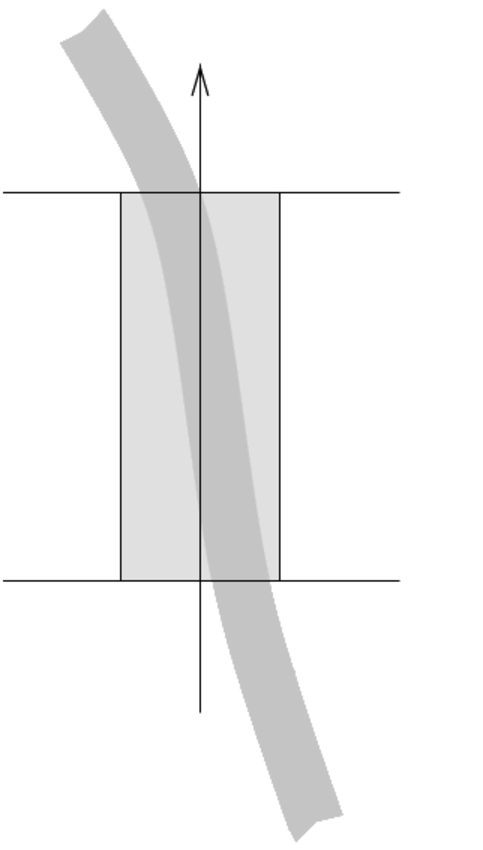
\includegraphics[scale=.4]{src/images/lbk-graphics/world-tube3.pdf}};
\node at (.45,0) {\small  $\gks$} ;
\node at (-.25,2.6) {\small  $ct$} ;
\node at (1.2,1.58) [right]{\small  $t=t_2$} ;
\node at (1.2,-1.11) [right]{\small  $t=t_1$} ;
\node at (-.38,-2.5) {\scriptsize  world tube} ;
\end{tikzpicture}
\end{center}
\caption{The world-tube of the material 
particle}\label{fig9.2}
\end{figure}
We push the lateral hyper-surface $\sigma$ to spatial 
infinity so that both the hyper-surfaces of constant time 
cover the whole of 3-space.

Now we observe that, in \eqref{rcm.22},  the  integral over 
$\sigma$ vanishes because  we assume $T^{\gka\gkb}\equiv 0$ 
on it. Then, we may rearrange \eqref{rcm.22}  as
\begin{align}\label{rcm.23}
\underset{t=t_1}{\int_{\text{all space}
\hspace{5mm}} \hspace{-15mm} T^{\gka0}dV} =
\underset{t=t_2}{\int_{\text{all
space} \hspace{5mm}}\hspace{-15mm}T^{\gka0}dV},
\end{align}
since $n_\gkb =\dow_\gkb t = (1,0,0,0)$ on the lid $t=$ 
constant $=t_2$ and, similarly $n_\gkb =(-1,0,0,0) $ on the 
lid $t=t_1$. Thus, the following 4-vector $P^\gka$ each 
component of which has the physical dimensions of momentum, 
is  {conserved} for the system: \index{continuous system ! 
conserved total 4-momentum}
\begin{align}\label{rcm.24}
P^\gka\equiv  \frac{1}{c}\int_{\text{all space}}
\hspace{-10mm} T^{\gka0}dV.
\end{align}
This conserved 4-vector $P^\gka$ is called the 
\textsl{conserved, total  4-momen\break tum of the {closed} 
system}.

\hbf{Physical meaning of the energy tensor components} 
\index{continuous system ! physical meaning of the energy 
tensor components} Observe that $P^\gka$ is  the (spatial) 
volume integral of $T^{\gka0}/c$. Therefore $T^{\gka0}/c$ 
may be identified as the \textsl{4-momentum density} of the 
system. Also, we note that
\begin{align}\label{rcm.25}
T^{00} =\eta^{00}\mtud{T}{0}{0}=\left\lbrace \frac{\dow
\qam }{\dow x^0} \frac{\dow \EuScript{L}}{\dow
\qgr{0}} - \EuScript{L}\right\rbrace \equiv\EuScript{W},
\end{align}
which is clearly is the \index{continuous system ! 
Hamiltonian density} \textsl{Hamiltonian density} (or 
energy density $\EuScript{W}$) of the system. Similarly we 
may find the  physical meaning of  the other components 
of the energy tensor. In this exercise, it is useful to 
note that all the components of the energy tensor have the 
dimension of energy density $(\SI{}{J/m^3})$.

Next, we consider the equation $\dow_\gkb T^{0\gkb}=0 $
written out in extenso:
\begin{align} \label{rcm.26}
0=\frac{\dow T^{00}}{\dow t} + \frac{\dow(c
T^{0i})}{\dow x^i}=\frac{\dow T^{00}}{\dow t} +
\vnab\dotp (cT^{0i}).
\end{align}
This being  a {continuity equation} for the energy density 
$T^{00}= \EuScript{W}$, implies that $c T^{0i}$, $i=1,2,3$, 
are the components of a {3-vector} representing the 
{energy-flux-density} in the system. Let  us define the 
3-vector  \index{continuous system ! energy-flux-density} 
\begin{align} \label{rcm.27} \vec{\EuScript{S}} \equiv 
(cT^{01},cT^{02},cT^{03}). \end{align} Note that the $i$-th 
components $c T^{0i} $, $i=1,2,3$, gives the amount of 
energy passing through unit area held  perpendicular to 
the $x^i$-direction.

To interpret the remaining nine components $ T^{ij}$,   
 $i,j=1,2,3$,  we appeal to the equations $\dow_\gka T^{i 
\gka} =0$ and note that it may be written as
\begin{align}\label{rcm.28}
&\dow_t (T^{i 0}/c) + \dow_j (T^{ij})=  \dow_t 
(\EuScript{S}^i/c^2)  + \dow_j T^{ij}\notag\\
& = \frac{\dow}{\dow t}(\EuScript{S}^i/c^2)  +
\nabla_jT^{ij}=0.
\end{align}
From these three continuity equations (one each for  
$i=1,2,3$), it follows that  $T^{ij}$ is the $j$-th 
component of  the flux of $\EuScript{S}^i /c^2 $. In other 
words, $T^{ij}$ is the density of momentum-flux in the $ 
x^j 
$-direction through a unit area held normal to the $ x^i 
$-direction. These nine components $T^{ij}$ form a second 
rank symmetric Cartesian tensor called the \textsl{stress 
tensor} of the system and is denoted by $\sigma^{ij}$. 
\index{continuous system ! stress tensor} Summarising,  we 
may display the energy tensor as follows:
\begin{align}\label{rcm.29}
T^{\gka\gkb}&=\begin{pmatrix}  T^{00}&T^{0i}\\
T^{i 0}&T^{ij}\end{pmatrix}  =\begin{pmatrix}
\EuScript{W}&
\vec{\EuScript{P}}\\
\vec{\EuScript{P}}&\sigma^{ij}\end{pmatrix} .
\end{align}

\section{The perfect fluid} \index{perfect fluid} 
The ideal or perfect fluid in special relativity is a  
continuous mechanical system described in a  Lorentz 
frame $S$ by the energy tensor \index{perfect fluid ! 
energy 
tensor} 
\begin{align}\label{rcm.30}
T^{\gka\gkb}&=(\rho_0 +p/c^2) U^\gka U^\gkb - p
\eta^{\gka\gkb},
\end{align}
where $\rho_0$ and $p$ are two \textsl{4-scalar fields} 
called the \textsl{density} and \textsl{pressure} of the 
fluid.  \index{perfect fluid ! density} \index{perfect 
fluid 
! pressure}The 4-scalar $\rho_0$ should be more 
appropriately called the \textsl{proper density of proper 
mass} of the  perfect fluid and is related to its 
\textsl{relative density of relative mass} $\rho$ by
\begin{align}\label{rcm.31}
\rho_0 &= (dm_0/dV_0) = (dm/ \Gamma)/(\Gamma
dV)=\Gamma^{-2}\rho,
\end{align}
Further, $U^\gka$ in Eqn.\eqref{rcm.30} is the 
\textsl{4-velocity field}\index{perfect fluid !  4-velocity 
field} of the   perfect fluid and is given by
\begin{align}\label{rcm.32}
U^\gka &=\Gamma\big(c,\vec{u}\big)\qquad
U_\gka  =\gky_{\gka\gkb}U^\gka=
\Gamma\big(c,-\vec{u}\big)
\end{align}
where
\begin{align}\label{rcm.33}
\Gamma \equiv (1-u^2/c^2)^{-1/2},
\end{align}
is the gamma-factor associated with particle 
\index{gamma-factor associated with a particle} 
3-velocity\footnote{Note that the $\Gamma(\vec{u})$ as well 
as the $\gamma(\vec{v})$ have the same functional form: 
however, $\Gamma(\vec{u})$ is associated with the particle 
3-velocity $\vec{u}$ in a given Lorentz frame whereas the 
familiar $\gamma(\vec{v})$ depends on the  inter-frame  
3-velocity $\vec{v}$.} field $\vec{u}=\vec{u}(x^\gka)$ of 
the 
fluid in the Lorentz frame $S$. Observe,
\begin{align}\label{rcm.34}
U^\gka U_\gka=\Gamma^2\big(c,\vec{u}\big)
\big(c,-\vec{u}\big)=\Gamma^2(c^2-u^2)=c^2.
\end{align}

We observe that dimensionally $U^\gka$ is a velocity, 
$\gky$ is dimensionless,
\begin{align*}
p&=\frac{\text{force}}{\text{area}} 
=\frac{\text{force}\times
\text{length}}{\text{volume}}=
\frac{\text{energy}}{\text{volume}}\\
&=\text{energy-density},
\end{align*}
so that $ (p/c^2) U^\gka U_\gkb $ is an energy-density. 
Therefore every component of the energy tensor 
\eqref{rcm.30} has the dimension of an energy-density.

Multiplying Eqn.\eqref{rcm.30} by $U_\gkb$ and using
Eqn.\eqref{rcm.33}, we get
\begin{align}\label{rcm.35}
T^{\gka\gkb}U_\gkb
&=(\rho_0 +p/c^2) U^\gka U^\gkb U_\gkb - p
\eta^{\gka\gkb} U_\gkb \\
&=c^2(\rho_0 +p/c^2)U^\gka -pU^\gka=\rho_0c^2U^\gka,
\end{align}
which shows that $ U^\gka$ is an eigenvector of 
$T^{\gka\gkb}$ belonging to the eigenvalue $\rho_0 c^2$. 
Multiplying this equation by $U_\gka$, again, we get
\begin{align}\label{rcm.36}
T^{\gka\gkb}U_\gka U_\gkb
&=(\rho_0 +p/c^2) U^\gka U^\gkb U_\gkb - p
\eta^{\gka\gkb} U_\gkb \\
&=c^2(\rho_0 +p/c^2)U^\gka -pU^\gka=\rho_0c^2.
\end{align}

We also note the useful relations
\begin{align} \label{rcm.37}
U_\gka (\dow_\gkb U^\gka)
=\frac{1}{2}\dow_\gkb(U_\gka U^\gka)
=\frac{1}{2}\frac{\dow c^2}{\dow x^\gkb}=0.
\end{align}
\begin{align} \label{rcm.38}
U^\gkm\dow_\gkm
=\rho_0 \frac{dx^\gkm}{d\gkt}
\frac{ \dow \;}{\dow x^\gkm}
=\frac{ \dd }{\dd \gkt},
\end{align}
where the second equation is valid along a world line
parametrized by the proper time $\gkt$ on it.

\section{Equations of motion for a perfect  fluid}
\index{perfect fluid ! equations of motion} 
For convenience, we break up  the perfect fluid energy 
tensor $T^{\gka\gkb}$ in Eqn.\eqref{rcm.30} as
\begin{align}\label{rcm.39}
T^{\gka\gkb}=\rho_0 U^\gka U^\gkb +S^{\gka\gkb},
\end{align}
where
\begin{align}\label{rcm.40}
S^{\gka\gkb}\equiv p(U^\gka U^\gkb/c^2
-\eta^{\gka\gkb}),
\end{align}
is called the {stress tensor}. Then, the equations
$\dow_\gkb T^{\gka\gkb}=0 $ read,
\begin{align}\label{rcm.41}
0=U^\gka\dow_\gkb (\rho_0 U^\gkb)
+\rho_0 U^\gkb (\dow_\gkb U^\gka)
+\dow_\gkb S^{\gka\gkb}.
\end{align}
Multiplying the above equation by  $U_\gka$, and using 
$U^\gka U_\gka=c^2$, we get
\begin{align}\label{rcm.42}
0= c^2 \dow_\gkb ( \rho_0U^\gkb)
+\rho_0 U^\gkb  U_\gka (\dow_\gkb U^\gka)
+U_\gka \dow_\gkb S^{\gka\gkb}.
\end{align}
Observe that  the second term on the right hand side  
vanishes because of Eqn.\eqref{rcm.37}. Therefore, 
Eqn.\eqref{rcm.42} may be rearranged as
\begin{align}\label{rcm.43}
 \dow_\gkb ( \rho_0U^\gkb)
=-c^{-2} U_\gka \dow_\gkb S^{\gka\gkb}.
\end{align}
Now, if we substitute for $\dow_\gkb (\rho_0 U^\gkb)$ from 
this equation back into Eqn.\eqref{rcm.41}, we get
\begin{align}\label{rcm.44}
0&=U^\gka\Big(-c^{-2}U_\gkm\dow_\gkn S^{\gkm\gkn}\Big)
+ \rho_0 U^\gkm \dow_\gkm U^\gka +
\dow_\gkm S^{\gka \gkm}.
\end{align}
We rearrange this equation as 
\begin{align} \label{rcm.45}
\rho_0 U^\gkm\dow_\gkm U^\gka
&=c^{-2}U^\gka U_\gkm
\dow_\gkn S^{\gkm\gkn}-
\dow_\gkn S^{\gka\gkn}\notag\\
&=\big(c^{-2}U^\gka U_\gkm-\mtud{\gkd}{\gka}{\gkm}
\big)\dow_\gkn S^{\gkm\gkn},
\end{align}
where we have changed the dummy $\gkm$ to $\gkn$ in the last
term.

Now, using Eqn.\eqref{rcm.38}, we rewrite the term on the 
left hand side of Eqn.\eqref{rcm.45} as
\begin{align} \label{rcm.46}
\rho_0 U^\gkm\dow_\gkm U^\gka
=\rho_0 \frac{\dd x^\gkm}{\dd \gkt}
\frac{ \dow U^\gka}{\dow x^\gkm}
=\rho_0 \frac{ \dd U^\gka}{\dd \gkt},
\end{align}
where $\dd \gkt=\dd s/c$ is the proper-time element on  
the  (timelike) world line (of a particle of the fluid) 
to which the 4-velocity $U^\gka=(\dd x^\gka/\dd \gkt)$ is a 
tangent and $(\dd U^\gka/\dd \gkt)$ is the 4-acceleration 
(on the particle's world line).  Plugging  
Eqn.\eqref{rcm.46} into Eqn.\eqref{rcm.45}, we finally 
obtain
\begin{align} \label{rcm.47}
\rho_0 \frac{\dd U^\gka}{\dd \gkt}
&=\big(c^{-2}U^\gka
U_\gkm-\mtud{\gkd}{\gka}{\gkm}
\big)\dow_\gkn S^{\gkm\gkn}.
\end{align}

Next, we calculate the term $\dow_\gkn S^{\gkm\gkn}$ in 
Eqn.\eqref{rcm.47}   explicitly: We have, using 
Eqn.\eqref{rcm.40},
\begin{align}\label{rcm.48}
\dow_\gkn S^{\gkm\gkn}
&=\dow_\gkn (p U^\gkm U^\gkn/c^2
-p\eta^{\gkm\gkn})\notag\\
&=(p/c^2)U^\gkn(\dow_\gkn U^\gkm)
+(p/c^2)U^\gkm (\dow_\gkn U^\gkn)\notag\\&\qquad
+(1/c^2)U^\gkm U^\gkn\dow_\gkn p
-\eta^{\gkm\gkn}(\dow_\gkn p)\notag\\
&=(p/c^2) (\dd U^\gkm/\dd \gkt) 
+(p/c^2) U^\gkm (\dow_\gkn U^\gkn)\notag\\&\qquad
+(1/c^2)U^\gkm U^\gkn\dow_\gkn p
-\eta^{\gkm\gkn}(\dow_\gkn p).
\end{align}
Plugging this into Eqn.\eqref{rcm.47}, we get,
\begin{scriptsize}\begin{align} \label{rcm.49}
&\rho_0 \frac{\dd U^\gka}{\dd \gkt}= 
\frac{U^\gka U_\gkm}{c^2}\Big\{ \frac{p}{c^2} \frac{\dd 
U^\gkm}{\dd \gkt} 
+\frac{pU^\gkm}{c^2} \frac{\dow U^\gkn}{\dow 
x^\gkn}
+\frac{U^\gkm U^\gkn}{c^2} \frac{\dow p\;\;}{\dow x^\gkn} 
-\eta^{\gkm\gkn} \frac{\dow p\;\;}{\dow x^\gkn}\Big\}
\notag\\
&\qquad\qquad -\mtud{\gkd}{\gka}{\gkm}\Big\{
\frac{p}{c^2}\frac{\dd U^\gkm}{\dd \gkt}  
+\frac{p}{c^2}U^\gkm \frac{\dow U^\gkn}{\dow x^\gkn}
+\frac{U^\gkm U^\gkn}{c^2} \frac{\dow p\;\;}{\dow x^\gkn}
-\eta^{\gkm\gkn}\frac{\dow p\;\;}{\dow x^\gkn}\Big\}.
\end{align}\end{scriptsize}
\nnnt Above, the first term on the right hand side 
vanishes  because
\begin{align}\tag{9.55b}
&U_\gkm\frac{\dd U^\gkm}{\dd\gkt}=\frac{1}{2}\frac{\dd 
(U_\gkm U^\gkm)}{\dd\gkt}=\frac{1}{2}\frac{\dd 
(c^2)}{\dd\gkt}=0.
\end{align} 
Also, the third  term on the right hand side cancels with 
the seventh.  Now,  replacing  $U_\gkm U^\gkm$ by $c^2$ and 
simplifying, equation \eqref{rcm.49} takes the form 
\begin{align}\label{rcm.50}
&\rho_0\frac{\dd U^\gka}{\dd\gkt\;\:}
= \frac{p U^\gka }{c^2}\frac{\dow U^\gkn}{\dow x^\gkn} 
-\frac{U^\gka U^\gkn }{c^2}\frac{\dow p\;\;}{\dow x^\gkn} 
\notag\\ &\qquad\qquad
-\frac{p}{c^2}\frac{\dd U^\gka}{\dd \gkt} 
-\frac{pU^\gka}{c^2} \frac{\dow U^\gkn}{\dow x^\gkn} 
+\eta^{\gka\gkn}\frac{\dow p\;\;}{\dow x^\gkn},
\end{align}
On cancelling off the first term   on the right hand side, 
with the fourth, and transferring the third term  to the 
left hand side, we may display Eqn. \eqref{rcm.50} as
\begin{align}\label{rcm.51}
\Big(\rho_0+ \frac{p}{c^2}\Big)
\frac{\dd U^\gka}{\dd \gkt\;\:}&=
\Big(-\frac{1}{c^2}U^\gka U^\gkn
+\eta^{\gka\gkn}\Big)\frac{\dow p\;\;}{\dow x^\gkn}.
\end{align}
If we express the factor $U^\gkn \frac{\dow p\;\;}{\dow 
x^\gkn}$ in the first term on the right hand side above as 
$\frac{\dd x^\gkn}{\dd\gkt\;\:}\frac{\dow p\;\;}{\dow 
x^\gkn}=\frac{\dd p} {\dd\gkt}$, we may  display 
Eqn.\eqref{rcm.51} in an equivalent form:
\begin{align}\label{rcm.52}
\Big(\rho_0+ \frac{p}{c^2}\Big)\frac{\dd 
U^\gka}{\dd\gkt\;\:}&=
-\frac{1}{c^2}U^\gka \frac{\dd p\,}{\dd\gkt} +
\eta^{\gka\gkn}\frac{\dow p\;\;}{\dow x^\gkn}.
\end{align}
Eqn.\eqref{rcm.51}, or its equivalent Eqn.\eqref{rcm.52}, 
give
 \textsl{the equations of motion for a perfect fluid in
special relativity}.

\exm Consider the 4-vector equation $A^\gka= B^\gka$ where 
the 4-vectors $A^\gka$ and $B^\gka$ are both orthogonal to 
a 
third 4-vector $X^\gka$. Prove that out of the set of four  
equations $A^\gka= B^\gka$, only three are independent. 
\soln We are given that
\begin{align*}
X_\gka A^\gka&=0=X_0 A^0+X_1 A^1+X_2 A^2+X_3 A^3,\\
X_\gka B^\gka&=0=X_0 B^0+X_1 B^1+X_2 B^2+X_3 B^3,
\end{align*}
which imply, for instance,
\begin{align*}
A^0&=-(X_1 A^1+X_2 A^2+X_3 A^3)/X_0=-(X_i A^i)/X_0,\\
B^0&=-(X_1 B^1+X_2 B^2+X_3 B^3)/X_0=(X_i B^i)/X_0.
\end{align*}
Now, using the {three} equations $A^i= B^i$, $i=1,2,3$,
we note that the fourth one follows as a consequence:
\begin{align*}
A^0&=-(X_i A^i)/X_0 =-(X_i B^i)/X_0=B^0,
\end{align*}
Thus, out of the four
equations $A^\gka= B^\gka$, only three are independent.
\ebxns

One can check [See example~9.4] that there are only {three 
independent equations} in Eqn.\eqref{rcm.51} (or its  
equivalent Eqn.\eqref{rcm.52}), because, on multiplying by 
$U_\gka$, both sides of Eqn.\eqref{rcm.51} vanish giving 
the 
identity $0=0$.

A fourth independent equation may be obtained as follows:
Multiplying Eqn.\eqref{rcm.48} by $U_\gkm$, gives
\begin{align*}
&U_\gkm\dow_\gkn S^{\gkm\gkn}=U_\gkm\dow_\gkn (p U^\gkm 
U^\gkn/c^2
-p\eta^{\gkm\gkn})\notag\\
&=(p/c^2)U_\gkm U^\gkn(\dow_\gkn U^\gkm)
+U_\gkm(p/c^2)U^\gkm (\dow_\gkn U^\gkn)\notag\\&\qquad
+(1/c^2)U_\gkm U^\gkm U^\gkn\dow_\gkn p
-U_\gkm \eta^{\gkm\gkn}(\dow_\gkn p)\notag\\
&=(p/c^2) U_\gkm (\dd U^\gkm/\dd \gkt) 
+p (\dow_\gkn U^\gkn)
+ U^\gkn(\dow_\gkn p) -U^\gkn(\dow_\gkn p).
\end{align*}
where, in the last step, we have used $U^\gkm U_\gkm=c^2$. 
Now, we note that the last two terms on the right hand side 
cancel each other while  $U_\gkm (\dd U^\gkm/\dd \gkt) =0$, 
(cf. Eqn. 9.55b),  so that the above equation becomes 
\begin{align}\label{rcm.62}
U_\gkm\dow_\gkn S^{\gkm\gkn}
&=p(\dow_\gkn U^\gkn),
\end{align}
where we have changed the dummy on the right hand side.
Plugging Eqn.\eqref{rcm.62} into Eqn.\eqref{rcm.43}, we get,
\begin{align}\label{rcm.63}
 \dow_\gkm (\rho_0 U^\gkm)
=-c^{-2}p(\dow_\gkn U^\gkn),
\end{align}
which may be expanded  as
\begin{align}\label{rcm.64}
U^\gkm \dow_\gkm \rho_0  + \rho_0 \dow_\gkm U^\gkm
=-c^{-2}p(\dow_\gkn U^\gkn).
\end{align}
Writing $U^\gkm \dow_\gkm \rho_0=(d\rho_0/d\gkt)$ and
collecting terms containing $\dow_\gkm U^\gkm$ together  in
Eqn.\eqref{rcm.64}, we get
\begin{align}\label{rcm.65}
\frac{\dd \rho_0}{\dd \gkt} +
\Big(\rho_0+\frac{p}{c^2}\Big)\dow_\gkm U^\gkm=0.
\end{align}
In equations \eqref{rcm.51} and  \eqref{rcm.65}, we have
five equations out of  which only four equations are
independent. Any four such independent equations give  the
equations of motion of a perfect fluid in special 
relativity.

\hbf{The Newtonian approximation of Eqn.\eqref{rcm.52}}
To carry out the approximation, we divide the equation
\eqref{rcm.52} by $\gkr_0$ and rearrange it as
\begin{align}\label{rcm.66}
\Big(1+ \frac{p}{\rho_0 c^2}\Big)\frac{\dd U^\gka}{\dd 
\gkt}&=
-\frac{1}{\rho_0 c^2}U^\gka \frac{\dd p}{\dd \gkt}
+\frac{1}{\rho_0}
\eta^{\gka\gkn}\frac{\dow p}{\dow x^\gkn}.
\end{align}
Then, we set
\begin{align*}
 \gkt\approx t , \quad \frac{p}{\gkr_0c^2}\frac{\dd 
U^\gka}{\dd \gkt}\approx 0\quad \text{ and} \quad 
\frac{1}{\rho_0 c^2}\frac{\dd p}{\dd \gkt}\approx 0
\end{align*}
in Eqn.\eqref{rcm.52} and obtain
\begin{align}\label{rcm.67}
\rho_0\frac{\dd U^\gka}{\dd t}&\approx
\eta^{\gka\gkb}\frac{\dow p}{\dow x^\gkb},
\end{align}
which is the required Newtonian approximation of  
Eqn.\eqref{rcm.52}. For $\gka=1,2,3$, Eqn.\eqref{rcm.67} 
may 
be expressed in 3-vector notation as
\begin{align}\label{rcm.68}
  \rho_0 \vec{a} =-\vnab p.
\end{align}
The other equation for $\gka=0$ in Eqn.\eqref{rcm.67} is 
an  approximate ``$0=0$ statement'' under the 
assumptions made (See the example 9.4 below).

\exmnp Prove that the $\gka=0$ equation in  \eqref{rcm.67}
is an approximate $0=0$ statement under the assumptions 
made.
\soln Setting $\gka=0$ in  Eqn.\eqref{rcm.67}, we get
\begin{align*}
 \gkr_0\frac{\dd U^0}{\dd \gkt}\approx\gky^{00}
 \frac{\dow p}{\dow (ct)}.
\end{align*}
Remembering that $\Gamma \approx 1$,  $\gkt\approx t$, 
$U^\gka\approx (c, \vec{u})$ in the Newtonian 
approximation, we write the above equation as
\begin{align*}
 \gkr_0\frac{\dd c}{\dd t}\approx\frac{1}{c}\frac{\dow 
p}{\dow t}.
\end{align*}
Clearly, the left hand side is zero and the right hand 
side is approximately zero under the Newtonian limit 
which is essentially a slow-motion, low-pressure limit. 
\\ \dm \hfill $\Box$

Next, we consider the Newtonian approximation of  the 
Eqn.\break \eqref{rcm.64}, i.e.,
\begin{align*}
U^\gkm \dow_\gkm \rho_0  + \rho_0 \dow_\gkm U^\gkm
=-c^{-2}p(\dow_\gkn U^\gkn).
\end{align*}
Neglecting the term on the right hand side as small,  we
write the above equation as
\begin{align}\label{rcm.69}
U^\gkm \dow_\gkm \rho_0  + \rho_0 \dow_\gkm U^\gkm
\approx 0.
\end{align}
Now, remembering that, in the Newtonian limit, $\Gamma 
\approx 1$,  $\gkt\approx t$, $U^\gka\approx (c, \vec{u})$, 
the above equation may be expanded and written as
\begin{align}\label{rcm.70}
c \frac{\dow \rho_0}{\dow (ct)}  +
\vec{u}\dotp\vnab\rho_0+\rho_0\frac{\dow c}{\dow
(ct)}+\rho_0\vnab\dotp \vec{u}\approx 0.
\end{align}
Clearly, the third term is zero here and we have,
\begin{align}\label{rcm.71}
\frac{\dow\rho_0}{\dow t} +
\vec{u}\dotp\vnab\rho_0+\rho_0\vnab\dotp
\vec{u}=\frac{\dow\rho_0}{\dow t} +  \vnab\dotp
(\rho_0\vec{u})\approx 0,
\end{align}
which is seen to be the familiar \textsl{continuity 
equation}.

In Eqns.\eqref{rcm.68} and \eqref{rcm.71}, we recognise the 
\textsl{Newtonian hydrodynamical equations for an ideal 
fluid free of  body-forces}.

\exm{Write down the ``energy tensor'' for a single 
point-particle and obtain the corresponding equation 
of motion.} \index{energy tensor for a single 
point-particle}
\soln In the incoherent matter energy tensor, we write 
$\rho_0 =m_0 \delta(x-x_0) \delta(y-y_0) \delta(z-z_0)$, 
where $\delta(x-x_0)$. $\delta(y-y_0)$ and $\delta(z-z_0)$ 
are  Dirac delta functions of their respective arguments 
and 
obtain,  \textsl{formally},  the energy tensor of a single 
particle. The 4-momentum of the particle is given by
\begin{align}\label{rcm.126}
P^i=\frac{1}{c}\int_{\text{all space}}
T^{i0}\dd V =\Gamma m_0 (c,\vec{u}),
\end{align}
and it is a constant 4-vector tangential to the world line 
of the particle. Its equation of motion is
\begin{align} \label{rcm.127}
\dd P^i/\dd \gkt =0.
\end{align}\ebxns
\section{Incoherent matter}\index{energy tensor ! 
incoherent matter}
Here, we describe a model a material continuum,  called 
an \textsl{incoherent matter} or, \textsl{incoherent  
fluid} which is  simply a perfect fluid with $p=0$. It 
is characterised 4-scalar  mass-density $\rho_0$, a 
4-velocity field $U^\gka$ and the energy tensor
\begin{align}\label{rcm.72}
T^{\gka\gkb}=\rho_0 U^\gka U^\gkb.
\end{align}
Writing
\begin{align}\label{rcm.73}
U^\gka = \Gamma  \dotup{x}{}^\gka
=\Gamma (\dd x^\gka/\dd t)=\Gamma(c,\vec{u}),
\end{align}
we get
\begin{align}\label{rcm.74}
T^{\gka\gkb}&= \rho_0 U^\gka U^\gkb  =\rho \dotup{x}{}^\gka
\dotup{x}{}^\gkb =\rho
\begin{pmatrix}
c^2 & c u_x & c u_y & c u_z\\
c u_x &  u_x u_x&u_x u_y& u_x u_z\\
c u_y &  u_y u_x & u_y u_y  & u_y u_z\\
c u_z &  u_z u_x & u_z u_y  & u_z u_z
\end{pmatrix} .
\end{align}
The equations $\dow_\gkb T^{\gka\gkb}=0 $ for the incoherent
fluid would then be
\begin{align} \label{rcm.75}
U^\gka\dow_\gkb (\rho_0 U^\gkb )
+(\rho_0 U^\gkb )\dow_\gkb U^\gka =0.
\end{align}
Contracting this with $U_\gka$ gives
\begin{align}\label{rcm.76}
\dow_\gkb (\rho_0 U^\gkb ) =0,
\end{align}
where we have used the result $U_\gka \dow_\gkb U^\gka =0$. 
Plugging Eqn.\eqref{rcm.76} back into Eqn.\eqref{rcm.75}, 
we 
get
\begin{align}\label{rcm.77}
\rho_0 (U^\gkb  \dow_\gkb) U^\gka
=\rho_0 (\dd U^\gka/\dd \gkt) =0,
\end{align}
where we have replaced $(U^\gkb \dow_\gkb)$ by $(\dd 
/\dd \gkt)$. 
This shows that the 4-acceleration of the particles of the 
incoherent fluid are zero, i.e., \textsl{there are no 
internal forces of any sort in the incoherent fluid}.

\section{The vacuum Maxwell field with  
sources}\index{vacuum Maxwell field with  sources}
The {Maxwell field is a 4-component continuous  
mechanical system}. The potentials $A_\gka  (x^\gkb)$ are 
the  field   amplitudes. The system Lagrangian in {SI 
units} is
\begin{align}\label{rcm.78}
\EuScript{L}=-\muo A_\gkm J^\gkm-\frac{1}{4}F_{\gkx\gky}
F^{\gkx\gky},
\end{align}
where $ F_{\gka\gkb}=\dow_\gka A_\gkb-\dow_\gkb A_\gka= 
A_{\gkb,\gka}-A_{\gka,\gkb}$,  with the comma denoting 
partial differentiation, and $ J^\gka=(c\rho,\vec{J}) $ is 
the  \textsl{4-current interacting with the Maxwell 
field}. \index{vacuum Maxwell field with sources ! 
4-current}

For the Lagrangian in Eqn.\eqref{rcm.78}, we have,
\begin{align}\label{rcm.79}
\frac{\dow\EuScript{L}\;\;\;}{\dow A_{\gka,\gkm}}
&=-2\cdot\frac{1}{4} F^{\gkx\gky}\:
\frac{\dow\phantom{A_{\gka,\gkm}}}
{\dow A_{\gka,\gkm}}(A_{\gky,\gkx} - A_{\gkx,\gky})\notag\\
&=-\frac{1}{2}F^{\gkx\gky}\,
(\delta_{\gky\gka}\delta_{\gkx\gkm} -
\delta_{\gkx\gka}\delta_{\gky\gkm})\notag\\&=
-\frac{1}{2} F^{\gkm\gka}+\frac{1}{2} F^{\gka\gkm}
=F^{\gka\gkm},\\\label{rcm.80}
\dow_\gkm\left(\frac{\dow\EuScript{L}\;\;\;\;}{\dow
A_{\gka,\gkm}}
\right)&= F^{\gka\gkm}_{\;\;\;,\gkm}; \quad
\frac{\dow\EuScript{L}\;}{\dow
A_\gka}=-\muo J^\gka.
\end{align}
Using these derivatives, we arrive at the Euler-Lagrange 
equations
\begin{align}\label{rcm.81}
\dow_\gkm F^{\gka\gkm}
\equiv F^{\gka\gkm}_{\;\;\;,\gkm}&=-\muo J^\gka,
\end{align}
which is \eqref{ved.38x} and, as we saw in \S8.6.2, is 
equivalent to the two Maxwell field equations \eqref{ved.1} 
and \eqref{ved.4} with the source terms.  It is important 
to note that the remaining two Maxwell  
equations\footnote{In the following chapter, we show that 
the two other Maxwell field equations, namely the  
equations 
\eqref{ved.2} and \eqref{ved.3}, called the {homogeneous  
equations},  are together equivalent to the tensor equation 
\eqref{rcm.86} which is also expressible as \eqref{rcm.87}. 
} \eqref{ved.2}, and  \eqref{ved.3} are \textbf{not} 
Euler Lagrange equations. They are automatically satisfied 
because $F_{\gka\gkb}$ is the \textsl{curl of a 
4-potential}.\index{vacuum Maxwell field ! 
4-potential}

\section{Charge in an external field} 
\index{equation of motion for a charge in an  external 
field}
In an inertial frame $S$, consider a system of $n$ 
electrically charged particles, of rest masses $m_i$ and 
charges $q_i$, all  interacting with one another. Let 
$F^{(e)}_{\gka\gkb}(\vec{r}_i,t)$ be the resultant 
electromagnetic field at the site $\vec{r_i}$ of the $i$-th 
charged particle at the instant $t$. The electromagnetic 
field  $F^{(e)}_{\gka\gkb}(\vec{r}_i,t)$ is determined by 
the positions and motions of the remaining $n-1$ particles 
$q_k,\;k\neq i$, of the system. However, such motions of 
the 
particles $q_k,\;k\neq i$, are affected by the position and 
motion of the $i$-th charged  particle $q_i$. Therefore, a 
consistent solution to the  problem seems almost 
impossible\footnote{See James L Anderson, 
\textit{Principles 
of Relativity Physics}, Academic Press, New York, 1967, 
p227, who observes as follows:  '\textsl{'In general, this 
task is beyond our abilities},...'' }. We proceed further 
by 
\textsl{assuming} that $F^{(e)}_{\gka\gkb}(\vec{r}_i,t)$ is 
a 
given function of the space and time coordinates in the 
region of interest\footnote{Effectively, this amounts to 
neglecting the influence of $q_i$ on the motion of the 
remaining $n-1$ charges $q_k,\;k\neq i$, of the 
system.}.  Then, we may, at least in principle, determine 
the  motion of $q_i$ provided we are given the field 
$F^{(e)}_{\gka\gkb}(\vec{r}_i,t)$ as a function of 
$(\vec{r}_i,t)$ in a certain region of interest.

The field $F^{(e)}_{\gka\gkb}(\vec{r}_i,t)$ in this problem 
is called the  \textsl{external field} acting on the 
charge $q_i$. Here, we may  recall the concept of a 
\textsl{test-charge} used to probe an  electromagnetic 
field. One may notice that the charge $q_i$ in this problem 
is in fact a test-charge which moves in the given external 
field $F^{(e)}_{\gka\gkb}(\vec{r}_i,t)$. From now on, to 
simplify the notation, we drop the superscript $(e)$ on 
$F^{(e)}_{\gka\gkb}(\vec{r}_i,t)$ and simply denote it by 
$F_{\gka\gkb}(\vec{r}_i,t)$ with the understanding that it 
represents the external field on $q_i$.

\subsection{The Heaviside-Lorentz ponderomotive\\ 
force} 
\index{Heaviside-Lorentz ponderomotive force}
In an inertial frame $S$, consider a particle of charge 
$q$  moving with the 4-velocity $U_\gkn$ in an external 
electro-magnetic field $F_{\gka\gkb}(\vec{r}_i,t)$. Then, 
the law of \textsl{ponderomotive} \footnote{From 
Wiktionary: Ponderomotive = The ability to move anything 
having a mass.} force due to  O. Heaviside and 
H.A.Lorentz states that the charged particle $q$ 
experiences a 
4-force (cf. Eqn.\eqref{pm50}) given by 
\begin{align}
 F^\gkm=F^{\gkm\gkn}J_\gkn=q F^{\gkm\gkn}U_\gkn.
\end{align}
Note that this 'law' gives a 4-force 
$F^{\gkm\gkn}$ under the assumption that  the 
electromagnetic field $F_q^{\gkm\gkn}$ due to $q$ 
\textsl{does not influence} the 
external field $F^{\gkm\gkn}$. Such an assumption  is 
usually referred to as the test-particle approximation for 
the interaction between the source-charges of the external 
field $F^{\gkm\gkn}$ and the  charge 
$q$.\index{test-charge}

\section{The source-free Maxwell field in\\ vacuum} 
\index{source-free Maxwell field in vacuum ! source-free}
In \S8.6, we saw that a {free  (i.e., source-free: $\rho=0, 
\; \vec{J}=0 $) electromagnetic field 
$\{\vec{E},\vec{B}\}$, 
in vacuum}, is described by the antisymmetric tensor
\begin{align}\label{rcm.83}
F^{\gkx\gky} =\begin{pmatrix}
 0       &   E_x/c  & E_y/c    & E_z/c\\
-E_x/c &   0        &  B_z      & -B_y\\
-E_y/c & - B_z     &  0         &  B_x\\
-E_z/c &   B_y     & -B_x      &  0\\
\end{pmatrix}.
\end{align}
We also recall that the covariant form of the above free 
field tensor is given by
\begin{align}\label{rcm.84}
F_{\gkx\gky} =\begin{pmatrix}
0      &   -E_x/c   & -E_y/c    & -E_z/c\\
E_x/c &   0         &  B_z       & -B_y\\
E_y/c & - B_z     &  0           &  B_x\\
E_z/c &   B_y     & -B_x        &  0\\
\end{pmatrix}.
\end{align}
Recall that the  free electromagnetic field in vacuum 
satisfies the  (source-free) Maxwell equations [see 
Eqns.\eqref{rcm.81} and  \eqref{ved.39x}]
\begin{align}\label{rcm.85}
\dow_\gky F^{\gkx\gky}&=0,
\end{align}
and
\begin{align}\label{rcm.86}
\dow_\gka F_{\gkb\gkg}
+\dow_\gkb F_{\gkg\gka}+\dow_\gkg F_{\gka\gkb} &=0,
\end{align}
where $\dual{F}^{\gkx\gky}$ is the {dual} Maxwell field
tensor. Eqn.\eqref{rcm.86} may also be expressed as
\begin{align}\label{rcm.87}
\dow_\gky(\dual{F}^{\gkx\gky})&=0,
\end{align}

\section{The energy tensor}\index{Maxwell energy tensor}
A symmetric  energy tensor of the (source) free Maxwell 
field, also called the \textsl{Maxwell energy tensor}, may 
be 
constructed following  the general methods described in 
\S9.3 and \S9.4. A suitable Lagrangian density for the 
free  Maxwell field is given by \index{Lagrangian density ! 
for the source-free Maxwell field}
\begin{align}\label{rcm.88}
 \EuScript{L}=-\frac{1}{4}F^{\gkl\gkr}F_{\gkl\gkr},
\end{align}
The free Maxwell field is a 4-component field and the field 
amplitudes $q_\gkm$ are the four potentials  
$A_\gkm(x^\gka)$. Therefore, the energy tensor of  the free 
Maxwell field is given by Eqn.\eqref{rcm.11} in which we 
write $q_\gkm=A_\gkm(x^\gka)$:
\begin{align}\label{rcm.89}
 ?T^\gka_\gkb? \equiv \frac{\dow A_\gkm}{\dow x^\gkb}
\frac{\dow \EuScript{L}}{\dow A_{\gkm,\gka}}
-?\delta^\gka_\gkb? \EuScript{L}=A_{\gkm,\gkb}
\frac{\dow \EuScript{L}}{\dow A_{\gkm,\gka}}
-?\delta^\gka_\gkb? \EuScript{L},
\end{align}
where we may recall that the notation $A_{\gkm,\gka}$ 
stands 
for 
the partial derivative $\dow_\gka A_{\gkm}\equiv (\dow 
A_{\gkm}/\dow x^\gka)$. 

\hbf{Construction and symmetrization} 
Differentiating $\EuScript{L}$  partially with respect to 
$A_{\gkm,\gka}$, we get
\begin{align}\label{rcm.90}
\frac{\dow \EuScript{L}}{\dow A_{\gkm,\gka}}
&=-\frac{1}{4}F^{\gkl\gkr}\frac{\dow F_{\gkl\gkr} }
{\dow A_{\gkm,\gka}}-\frac{1}{4}F_{\gkl\gkr}\frac{\dow
F^{\gkl\gkr} }{\dow A_{\gkm,\gka}}\notag\\
&=-\frac{1}{2}F^{\gkl\gkr}\frac{\dow F_{\gkl\gkr} } {\dow 
A_{\gkm,\gka}}=-\frac{1}{2}F^{\gkl\gkr}\frac{\dow(A_{\gkr, 
\gkl} -A_{\gkl,\gkr})} {\dow A_{\gkm,\gka}}\notag\\
&=-\frac{1}{2}F^{\gkl\gkr}
\Big(?\delta^\gkm_\gkr? 
?\delta^\gka_\gkl?-?\delta^\gkm_\gkl?
?\delta^\gka_\gkr?\Big)\notag\\
&=-\frac{1}{2}F^{\gka\gkm}
+\frac{1}{2}F^{\gkm\gka}=F^{\gkm\gka}.
\end{align}
Plugging this into Eqn.\eqref{rcm.89}, we get 
\begin{align}\label{rcm.91}
?T^\gka_\gkb?
=A_{\gkm,\gkb}F^{\gkm\gka}
+\frac{1}{4}?\delta^\gka_\gkb? 
F^{\gkl\gkr}F_{\gkl\gkr}
\end{align}
We follow the method described in \S9.4 and symmetrize this
tensor. To this end, we consider the tensor
\begin{align}\label{rcm.92}
?{\psi}_{\gkb}^{\gkm\gka}? 
\equiv ?A_{\gkb}??F^{\gkm\gka}?,
\end{align}
which satisfies the two requirements
\begin{align}\label{rcm.93}
&?{\psi}_{\gkb}^{\gkm\gka}? \equiv
?A_{\gkb}??F^{\gkm\gka}?=-?A_{\gkb}? 
?F^{\gka\gkm}?=-?{\psi}_{ \gkb }^{\gka\gkm}?, \quad 
\text{and}\notag\\
&\Big(?{\psi}_{\gkb}^{\gkm\gka}?\Big)_{,\gkm\gka}=0.
\end{align}
It has a divergence,
\begin{align}\label{rcm.94}
?{\psi}_{\gkb}^{\gkm\gka}?_{,\gkm}=?A_{\gkb,\gkm}?
?F^{\gkm\gka}?+?A_{\gkb}? ?F^{\gkm\gka}?_{,\gkm}
=?A_{\gkb,\gkm}? ?F^{\gkm\gka}?,
\end{align}
which follows because of the free-field Maxwell equation 
$?F^{\gkm\gka}?_{,\gkm}$=0. Adding
$?{\psi}_{\gkb}^{\gkm\gka}?_{,\gkm}=A_{\gkb,\gkm}
?F^{\gkm\gka}?=-A_{\gkb,\gkm}
?F^{\gka\gkm}?$ to the energy tensor in \eqref{rcm.91}, we 
get
\begin{align}\label{rcm.95}
?T^\gka_\gkb? &=F^{\gka\gkm}\Big(A_{\gkm,\gkb}
-A_{\gkb,\gkm}\Big) +\frac{1}{4}?\delta^\gka_\gkb?
F^{\gkl\gkr}F_{\gkl\gkr}\notag\\
&=F^{\gka\gkm}F_{\gkb\gkm}
+\frac{1}{4}?\delta^\gka_\gkb? F^{\gkl\gkr}F_{\gkl\gkr}.
\end{align}
That this tensor is unchanged when the indices $\gka$ and 
$\gkb$ are interchanged is not obvious from its expression 
above. However, a look at the explicit expressions for 
these  components shows that it is, 
indeed,so\footnote{Here, we wish to mention that a symmetry 
with respect to a pair of unlike indices is not a tensor 
symmetry (See Example~9.3). Under a general coordinate 
transformation, the relation $?T^\gka_\gkb? =?T^\gkb_\gka?$ 
{does not} guarantee  the relation $?T^\gka'_\gkb'? 
=?T^\gkb'_\gka'?$. However, under a Lorentz transformation 
this symmetry is preserved and in all Lorentz frames, 
$?T^\gkb_\gka?$ in Eqn.\eqref{rcm.97} is symmetric.}. A 
direct  calculation (see Example~9.5) yields
\begin{align}\label{rcm.96}
&\mtud{T}{0}{0}=\frac{1}{2}\left(\eps_0
E^2+B^2/\muo\right)=\EuScript{W}, \\ \label{rcm.97}
&\mtud{T}{0}{k} =-(\vec{E}\times\vec{B})_k/\muo c= -S_k/c=
\mtud{T}{k}{0}, \\ \label{rcm.98}
&\mtud{T}{k}{m}
=\epso(E_k E_m -\mtud{\delta}{k}{m}E^2/2)\notag\\
&\qquad +(B_k B_m -\mtud{\delta}{k}{m}
B^2/2)/\muo=\mtud{T}{m}{k},
\end{align}
which show that  $\mtud{T}{\gka}{\gkb}$ is symmetric in 
$\gka$ and $\gkb$. In these formulae, we may note that (see 
Eqns.\eqref{rcm.25} and  \eqref{rcm.27} of \S9.7)
\begin{align}\label{rcm.99}
\EuScript{W}\equiv\frac{1}{2}\left(\eps_0
E^2+B^2/\muo\right),
\end{align}
is the \textsl{energy density} of the free electromagnetic 
field and the 3-vector \index{source-free electromagnetic 
field ! energy density}
\begin{align}\label{rcm.100} 
\vec{\EuScript{S}}\equiv\frac{1}{\muo}\vec{E}\times\vec{B} 
=\Big(\EuScript{S}_1,\,\EuScript{S}_2,\,\EuScript{S}_3\Big),
 \end{align} 
represents the  \textsl{energy-flux-density} and is called 
\textsl{Poynting  3-vector} of the free electromagnetic 
field. \index{Poynting 3-vector}

Lastly, from Eqn.\eqref{rcm.26}, we note the conservation 
law
\begin{align} \label{rcm.101}
0=\frac{\dow T^{00}}{\dow t} + \frac{\dow(c
T^{0i})}{\dow x^i}=\frac{\dow\EuScript{W}}{\dow t} +
\vnab\dotp \EuScript{S},
\end{align}
which is the \textsl{continuity equation} for the energy
density $\EuScript{W}$ of the free electromagnetic field.
\index{source-free electromagnetic 
field ! continuity equation} 

Raising the index $\gkb$ in \eqref{rcm.95} we obtain  the
$(2,0)$-form, or the pure-contravariant form of the
Maxwell energy  tensor:
\begin{align}\label{rcm.102}
\muo T^{\gka\gkb}&=-F^{\gka\gkm}\mtud{F}{\gkb}{\gkm}
+\frac{1}{4}F^ {\gkm\gkn} F_{\gkm\gkn}
\,\gky^{\gka\gkb}\notag\\
&=-\gky_{\gkm\gkn}F^{\gka\gkm}F^{\gkb\gkn}
+\frac{1}{4}(F^ {\gkm\gkn} F_{\gkm\gkn})
\,\gky^{\gka\gkb}.
\end{align}
Using \eqref{rcm.96}-\eqref{rcm.98}, we obtain, after a 
little rearrangement,
\begin{align}\label{rcm.103}
&T^{00}=\gky^{00}\mtud{T}{0}{0}=\EuScript{W}\notag,\\
&T^{0k}=\gky^{kk}\mtud{T}{0}{k}=-\mtud{T}{0}{k}=
+S_k/c= T^{k 0},\notag \\
&T^{km}= \epso\left\lbrace E_k E_m
-\mtud{\delta}{k}{m} E^2/2\right \rbrace \notag\\
&\qquad +(1/\muo)\left\lbrace
B_k B_m -\mtud{\delta}{k} {m} B^2/2\right\rbrace=T^{mk}.
\end{align}
where $k,m=1,2,3$. Clearly, this tensor is symmetric. The 
nine components $T^{km}$ form a second rank symmetric 
Cartesian 3-ten-\break sor called the \textsl{Maxwell stress 
tensor} 
\index{Maxwell stress tensor}
which we denote by $\boldsymbol{\sigma}^{\alpha \beta}$. 
The 
contravariant Maxwell energy tensor may also be displayed 
in 
block-matrix form as
\begin{align}\label{rcm.104}
\EuScript{T}^{\alpha \beta}
=\begin{pmatrix}
\EuScript{W} & \vec{S}/c\\
\vec{S}/c&\boldsymbol{\sigma}^{\alpha \beta}
\end{pmatrix}.
\end{align}

\exmnp Calculate the mixed components $\mtud{T}{\gka}{\gkb}$
of the free  electromagnetic energy tensor.
\soln  Using Eqns.\eqref{rcm.83} and \eqref{rcm.84}, we
have
\begin{align}\label{rcm.117}
F^ {\gkm\gkn} F_{\gkm\gkn}& =2(B^2-E^2/c^2).
\end{align}
Using Eqns.\eqref{rcm.83}, \eqref{rcm.84} and
\eqref{rcm.98} in  Eqn.\eqref{rcm.70}, we then get
\begin{align*}
&\muo\mtud{T}{0}{0}
=-(F^{01}F_{01}+F^{02}F^{02}+F^{03}F_{03})\notag\\
&\qquad\qquad+\frac{1}{4}2\left(E^2/c^2+B^2\right)
\mtud{\gkd}{0}{0 } \notag\\
& =-(-E_x^2/c^2-E_y^2/c^2-E_z^2/c^2)+\frac{1}{2}
\left(E^2/c^2+B^2\right)\notag\\
& =\frac{1}{2}\left(E^2/c^2+B^2\right)
=\frac{1}{2}\left(\eps_0\muo E^2+B^2\right),
\end{align*}
so that
\begin{align}\label{rcm.118}
\mtud{T}{0}{0}&=\frac{1}{2}\left(\eps_0
E^2+B^2/\muo\right)=\EuScript{W},
\end{align}
is the energy density of the free electromagnetic field.  
Next, we note that
\begin{align}
&\nnnt\nnnt   \muo\mtud{T}{0}{1}
=-(F^{00}F_{01}+F^{01}F_{11}+F^{02}F_{21}
+F^{03}F_{31}) \notag\\&\nnnt\nnnt +\frac{1}{2}\left(E^2/c^2
+B^2\right)
\,\mtud{\gkd}{1}{0}=-E_y B_z/c+E_z
B_y/c\notag\\&=-\frac{1}{c}(\vec{E}\times
\vec{B})_x,\notag\\
&\nnnt\nnnt\text{which gives
}\;\mtud{T}{0}{1}=-\frac{1}{c}\EuScript{S}_1
=\mtud{T}{1}{0},
\end{align}
where $\EuScript{S}_1$ is the $x$-component of the Poynting 
vector  defined in Eqn.\eqref{rcm.97}. From this, we may 
easily guess the general formula
\begin{align}\label{rcm.120}
\mtud{T}{0}{k}&= \mtud{T}{k}{0} = -S_k/c, \quad
k=1,2,3.
\end{align}
Similarly,  we obtain, for $k,m=1,2,3$,
\begin{align}\label{rcm.121}
\mtud{T}{k}{m}=\mtud{T}{m}{k}
&=\epso(E_k E_m 
-\mtud{\delta}{k}{m}E^2/2)\notag\\&\qquad+(B_k
B_m -\mtud{\delta}{k}{m} B^2/2)/\muo.
\end{align}\ebxns

\exm Verify explicitly that the energy tensor of the free 
Maxwell field has zero trace, i.e., \index{source-free 
Maxwell field ! trace of the energy tensor}
$\mtud{T}{\gka}{\gka}=0$. \soln From Eqn.\eqref{rcm.121}, 
we have
\begin{align}\label{rcm.122}
\mtud{T}{1}{1}&
=\epso(E_1^2 -\mtud{\delta}{1}{1}E^2/2)+(B_1^2
-\mtud{\delta}{1}{1} B^2/2)/\muo \notag \\
&=\epso(E_1^2 -E^2/2)+(B_1^2-B^2/2)/\muo \notag\\
&=\frac{\epso}{2}
(E_1^2-E_2^2-E_3^2)+\frac{1}{2\muo}
(B_1^2-B_2^2-B_3^2).
\end{align}
Similarly, we obtain
\begin{align}\label{rcm.123}
\mtud{T}{2}{2}=\frac{\epso}{2}
(E_2^2-E_3^2-E_1^2)+\frac{1}{2\muo}
(B_2^2-B_3^2-B_1^2).
\end{align}
\begin{align}\label{rcm.124}\mtud{T}{3}{3}
=\frac{\epso}{2}
(E_3^2-E_1^2-E_2^2)+\frac{1}{2\muo}
(B_3^2-B_1^2-B_2^2).
\end{align}
Adding Eqns. \eqref{rcm.118}, \eqref{rcm.122}, 
\eqref{rcm.123}
and \eqref{rcm.124}, we get
\begin{align}\label{rcm.125}
&\tr{T} =\frac{\epso}{2} (E_1^2+E_2^2+E_3^2)
+\frac{1}{2\muo} (B_1^2+B_2^2+B_3^2)\notag\\
&\;+\frac{\epso}{2}
(E_1^2-E_2^2-E_3^2)+\frac{1}{2\muo}
(B_1^2-B_2^2-B_3^2)\notag\\
&\;+\frac{\epso}{2}
(E_2^2-E_3^2-E_1^2)+\frac{1}{2\muo}
(B_2^2-B_3^2-B_1^2)\notag\\
&\;+\frac{\epso}{2}(E_3^2-E_1^2-E_2^2)
+\frac{1}{2\muo} (B_3^2-B_1^2-B_2^2)=0.
\end{align} \ebxns

\section{Canonical form of the energy tensor}
\index{Maxwell energy tensor ! Canonical forms}
\hbf{The non-null case} We may recall Rainich theorem of 
\S~8.5.4: According to this theorem, a non-null Maxwell 
field at an event $P$ may be reduced to an electromagnetic 
wrench by transforming to a suitable Lorentz frame, say 
$S$, 
at $P$. Further, by rotating the spatial axes of $S$ till 
the 3-vectors $\vec{E}$ and $\vec{B}$ of the wrench have 
only 
their  $z$-components non-zero, the tensor $F_{ab}(P)$ 
assumes the following canonical form 
\begin{align}\label{rcm.117x}
F_{\gka\gkb}=\begin{pmatrix}
 0  & 0 & 0 & -E_z/c\\
0 & 0  & B_z  & 0\\
0 & - B_z  & 0   & 0\\
E_z/c & 0  & 0  & 0\\
\end{pmatrix}.
\end{align}
If we put $E_x=E_y=B_x=B_y=0$ in the formulae of 
Example~9.6, we get the following diagonal Maxwell energy 
tensor for the field tensor $F_{ab}$ in 
Eqn.\eqref{rcm.117x}:
 \begin{align}\label{rcm.105}
\mtud{T}{\gka}{\gkb}=\begin{pmatrix}
\mtud{T}{0}{0}  & 0 & 0  & 0\\
0  & \mtud{T}{1}{1} &0 & 0\\
0 & 0 & \mtud{T}{2}{2} &  0 \\
0 &   0     &   0    & \mtud{T}{3}{3}
\end{pmatrix}
\end{align}
where
\begin{align}\label{rcm.106}
\mtud{T}{0}{0}&=\epso E_z^2/2+B_z^2/2\muo,\\\label{rcm.107}
\mtud{T}{1}{1}&=-\epso E_z^2/2-B_z^2/2\muo,\\\label{rcm.108}
\mtud{T}{2}{2}&=-\epso E_z^2/2-B_z^2/2\muo,\\\label{rcm.109}
\mtud{T}{3}{3}&=\epso E_z^2/2+B_z^2/2\muo.
\end{align}
Evidently, this diagonal tensor has zero trace, i.e.,  
$\mtud{T}{\gka}{\gka}=0$.

\hbf{The null case}
There is not much one can do by performing a Lorentz boost 
to simplify the a null  electromagnetic energy tensor at 
an event. However, we have seen that we may bring it to the 
canonical form \eqref{ved.60x} by performing a suitable 
spatial rotation on the null  electromagnetic field 
tensor at $P$. Using this tensor,  \ie, Setting 
$E_x=E_z=B_x=B_y$ in the formulae of Example~9.6, we obtain 
the following (non-diagonal) canonical energy tensor 
representing a null Maxwell field at an event:
\begin{align}\label{rcm.110}
\mtud{T}{\gka}{\gkb}
=\begin{pmatrix}
\mtud{T}{0}{0}  & \mtud{T}{0}{1} & 0  & 0\\
\mtud{T}{1}{0}  & \mtud{T}{1}{1} &0 & 0\\
0 & 0 & \mtud{T}{2}{2} &  0 \\
0 &   0     &   0    & \mtud{T}{3}{3}
\end{pmatrix}
\end{align}
where
\begin{align}\label{rcm.111}
\mtud{T}{0}{0}&=+\epso E_y^2/2+B_z^2/2\muo,
\\\label{rcm.112}
\mtud{T}{1}{1}&=-\epso E_y^2/2-B_z^2/2\muo,
\\\label{rcm.113}
\mtud{T}{2}{2}&=+\epso E_y^2/2-B_z^2/2\muo,
\\\label{rcm.114}
\mtud{T}{3}{3}&=-\epso E_y^2/2+B_z^2/2\muo,
\end{align}
\begin{align}\label{rcm.115}
\mtud{T}{0}{1}&=\mtud{T}{1}{0}
=-\frac{1}{c}(\vec{E}\times \vec{B})_x.
\end{align}
It is easily checked that this canonical tensor too has zero
trace, i.e., $\mtud{T}{\gka}{\gka}=0$.
%~ \newpage
\section*{Appendix 9A: The chain rule of partial\\  
differentiation}

\hbf{Chain rule: Single independent variable}\\ Let 
$L=f(q,\dot{q},t)$ where $q=q(t)$, $\dot{q}=\dot{q}(t)$ 
are  differentiable functions of the single independent 
variable $t$. Then, the chain rule for $(\dd L/\dd t)$ is 
given by
\begin{align}\label{128}
\dod{L}{x}
&=\dpd{f}{q}\dod{q}{t}+\dpd{f}{\dot{q}}\dod{\dot{q}}{t}
+\dpd{f}{t}\dod{t}{t}\notag\\
&=\dpd{f}{q}\dod{q}{t}+\dpd{f}{\dot{q}}\dod{\dot{q}}{t}
+\dpd{f}{t}.
\end{align}
\hbf{Chain rule: Many independent variables} For the sake 
simplicity, we consider here the case of two independent 
variables, namely $x$ and $t$. Let 
$\EuScript{L}=f(q,\dot{q},x,t)$ where  $q$ and $\dot{q}$ 
are 
two differentiable functions of $x$ and $t$. Then, the 
chain 
rule for the partial derivatives $\dpd{\EuScript{L}}{x}$ 
and $\dpd{\EuScript{L}}{t}$ are as follows:
\begin{align}\label{129}
\dpd{\EuScript{L}}{x}
&=\dpd{f}{q}\dpd{q}{x}+\dpd{f}{\dot{q}}\dpd{\dot{q}}{x}
+\dpd{f}{x}\dpd{x}{x}\notag\\ 
&=\dpd{f}{q}\dpd{q}{x}
+\dpd{f}{\dot{q}}\dpd{\dot{q}}{x} +\dpd{f}{x},
\end{align}
\begin{align}
\dpd{\EuScript{L}}{t}&=\dpd{f}{q}\dpd{q}{t}+\dpd{f}{
\dot {q}}
\dpd{\dot{q}}{t} +\dpd{f}{t}\dpd{t}{t} \notag\\
&=\dpd{f}{q}\dpd{q}{t}+\dpd{f}{\dot{q}} 
\dpd{ \dot{q}}{t} +\dpd{f}{t},\label{130}
\end{align}
These rules apply even if one, or, both, the functions 
$q$ and $\dot{q}$ are not functions of $x$ and/or $t$. 
Then, we need only set the corresponding partial 
derivatives equal to zero in the chain rule\footnote{We 
urge the reader to refer to the Classic: Lipman Bers, 
\textsl{Calculus}, 1969, Vol II, p. 804, Holt, Reinhart 
and Winston, Inc.}.

\exm Verify the chain rule for the function  
$L(q,\dot{q},t) =q^2+(\dot{q})^2+e^{-t}$  where  
$q(t)=\sin(t)$. \soln Plugging $q(t)=\sin(t)$ and 
$\dot{q}(t)=\cos(t)$ into $L$, we get
\begin{align}\label{131}
L(t)&=q^2+(\dot{q})^2+e^{-t}\notag\\&
=\sin^2(t)+\cos^2(t)+e^{-t}=e^{-t}.
\end{align}
Therefore,
\begin{align}\label{132}
\dod{L}{t}&=-e^{-t}.
\end{align}
Also, we have,
\begin{align*}\quad \dpd{L}{q} =2q , \quad
\dpd{L}{\dot{q}}=2\dot{q},\quad \dpd{L}{t}=-e^{-t}.
 \end{align*}
Using these in the chain rule for $L$, we get
\begin{align} \label{133}
 \dod{L}{t}&=\dpd{L}{q}\dpd{q}{t}
+\dpd{L}{\dot{q}}\dpd{\dot{q}}{t}+\dpd{L}{t}\notag\\
&=2q\cos(t)+2\dot{q}[-\sin(t)]-e^{-t}=-e^{-t},
\end{align}
which agrees with \eqref{132} thus verifying the chain rule.

\exm Similarly, verify the chain rule for  
$L=f(q,\dot{q},x,t) \break =q+\dot{q}+tx$ where  $q(x,t)=x\sin(t)$.
\soln First, substituting for $q$ and $\dot{q}$ explicitly 
into $L$, we express $L$ as a function of the independent 
variables $x$ and $t$:
\begin{align}\label{134}
L=x \sin (t)+x\cos(t)+tx.
 \end{align}
Differentiating this partially with respect to $x$ and $t$, 
we get
\begin{align}\label{135}
&\dpd{L}{x}=\sin (t)+\cos(t)+t,\\\label{136}
&\dpd{L}{t}=x\cos(t)-x\sin(t)+x.
 \end{align}
Formally, the chain rules for $\pd{L}{x}$ and $\pd{L}{t}$ 
are
\begin{align}\label{137}
\dpd{L}{x}=\dpd{f}{q}\dpd{q}{x}+\dpd{f}{\dot{q}}
\dpd{\dot{q}}{x}+\dpd{f}{x},\\\label{138}
\dpd{L}{t}=\dpd{L}{q}\dpd{q}{t}+\dpd{L}{\dot{q}}
\dpd{\dot{q}}{t}+\dpd{f}{t}.
\end{align}
Plugging $\pd{f}{q}=1$, $\pd{f}{\dot{q}}=1$, 
$\pd{q}{x}=\sin(t)$, $\pd{\dot{q}}{x}=\cos(t)$ and 
$\pd{f}{x}=t$ into Eqn.\eqref{138} above, we get
\begin{align}\label{139}
 \dpd{L}{x}&= 1.\sin(t)+1.\cos(t)+t,
 \end{align}
which agrees with Eqn.\eqref{135} thus verifying the chain 
rule \eqref{137}. Similarly, one may verify the chain rule 
\eqref{138} also.
\hbf{Note} If we had used the \textbf{sloppy notation} 
$L=L(q,\dot{q},x,t)  =q+\dot{q}+tx$ in this example, the 
chain rules Eqn.\eqref{137} and  Eqn.\eqref{138} would 
appear as
\begin{align*}
\dpd{L}{x}=\dpd{L}{q}\dpd{q}{x}+\dpd{L}{\dot{q}}
\dpd{\dot{q}}{x}+\dpd{L}{x},\\
\dpd{L}{t}=\dpd{L}{q}\dpd{q}{t}+\dpd{L}{\dot{q}}
\dpd{\dot{q}}{t}+\dpd{L}{t},
\end{align*}
and the identical-looking terms on either side of these 
equations are not to be cancelled-off, which is very 
confusing. The trouble is due to the sloppy notation that 
we 
used. If we insist on using the customary sloppy notation, 
then, we must mark the term $\pd{L}{x}$ and $\pd{L}{t}$ on 
the right hand sides of the above chain rules, as, say, 
$\frac{\dow' L}{\dow x}$ and $\frac{\dow' L}{\dow t}$, and 
explain why we did so. We have done  precisely that in 
Eqn.\eqref{rcm.7}.

\section*{Exercises}
\exise If $?T^{\gka}_{\gkb}?$ is a mixed tensor, show that 
the relation  $?T^{\gka}_{\gkb}?=?T_{\gkb}^{\gka}?$, 
although may be true in in one coordinate system,  in 
general, is not true in some other allowed coordinate 
system. However, a symmetry of a tensor with respect a pair 
of like (contravariant, or covariant) indices is carried 
over to all allowed coordinate systems. If, 
$?T_{\gka\gkb}?=?T_{\gkb\gka}?$ is a symmetric tensor, for 
example, then $?T_{\gka\gkb}?=?T_{\gkb\gka}? 
\Leftrightarrow ?T_{\gka'\gkb'}?= ?T_{\gkb'\gka'}?$.

\exise Obtain the equations for the following systems from 
a 
variational principle: (a).\ Real scalar  field, (b).\ 
Complex scalar field (c).\ Schrodinger field, and (d).\  
Dirac field.

\exise Prove the equations \eqref{rcm.86} and
\eqref{rcm.87} are the same.

\begin{small}
\begin{quote}
{References}

[1] L D Landau and E M Lifshitz, \textsl{The Classical 
Theory of Fields}, Fourth Revised English Edition, Course of 
Theoretical Physics Volume 2, Chapters 3 and 4, pp. 43-85

[2] A O Barut, \textsl{Electrodynamics and Classical  
Theory of Fields, and Particles},  Chapter III,  pp. 
85-95

[3] J L Synge, \textsl{Relativity :  The Special 
Theory},  North Holland Publishing Company, Amsterdam, 
1972,  Chapter VIII. 

[4] J L Synge, \textsl{Relativity :  The General 
Theory},   North Holland Publishing Company, Amsterdam, 
1971,  Chapter IV, Section 4.
\end{quote}
\end{small}
